\documentclass[11pt,letterpaper]{article}

%%%%%%%%%%%%%%%%%%%%%%%%%%%%%%
\pagestyle{plain}                                                      %%
%%%%%%%%%% EXACT 1in MARGINS %%%%%%%                                   %%
\setlength{\textwidth}{6.5in}     %%                                   %%
\setlength{\oddsidemargin}{0in}   %% (It is recommended that you       %%
\setlength{\evensidemargin}{0in}  %%  not change these parameters,     %%
\setlength{\textheight}{9.0in}    %%  at the risk of having your       %%
\setlength{\topmargin}{0in}       %%  proposal dismissed on the basis  %%
\setlength{\headheight}{0in}      %%  of incorrect formatting!!!)      %%
\setlength{\headsep}{0in}         %%                                   %%
\setlength{\footskip}{.5in}       %%                                   %%

%%%%%%%%%%%%%%%%%%%%%%%%%%%%%%%%%%%%                                   

\usepackage[pdftex]{graphicx}
\usepackage{color}
\usepackage{url}
\usepackage{tabularx}
\usepackage{tikz}

% From PPoPP
\usepackage{amsmath}
\usepackage{amsfonts}
%\usepackage{graphicx}
%\usepackage{xspace}
\usepackage{verbatim}
%\usepackage{listings}
\usepackage{multirow}
\usepackage{subfigure}
\usepackage{pdfpages}
%% % Tweak spacing to fit in page limit if needed
%% % ============================================
%% % gap between text and figs/tables:
%% \addtolength\textfloatsep{-0.2in}
%% % gap between figs/tables and other figs/tables
%% \addtolength\floatsep{-0.1in}
%% % gap between figure and caption
%% \addtolength\abovecaptionskip{-0.05in}
%% \addtolength\intextsep{0in}

\hyphenation{ }

\setlength{\parindent}{0.5cm}

\newif\ifdraft
% comment out the next line to turn off comments
%\drafttrue

\ifdraft
  \definecolor{darkgreen}{rgb}{0,0.5,0}
  \newcommand{\manish}[1]{ {\it \color{red} \{#1 -Tahsin\}}}
  \newcommand{\hasan}[1]{ {\textcolor{blue} { #1 -Hasan }}}
  \definecolor{orange}{rgb}{0.7,0.5,0.0}
  \newcommand{\klasky}[1]{{\textcolor{orange}{ #1 -Scott }}}
  % Red star denotes items that need further work or discussion
  \newcommand{\TODO}[1]{{\textcolor{red}{ TO DO: #1 }}}
\else
  \newcommand{\klasky}[1]{}
  \newcommand{\hasan}[1]{}
\fi

%\newcommand{\ititle}{\textsc{\textbf{HESK}}}
\newcommand{\ititle}{\textsc{HESK}}
\newcommand{\insitu}{\textit{in situ }}

\let\oldenumerate\enumerate
\renewcommand{\enumerate}{
      \oldenumerate
      \setlength{\itemsep}{1pt}
      \setlength{\parskip}{0pt}
      \setlength{\parsep}{0pt}
}

% A definition we do not want the reader to forget
\newcommand{\defn}[1] {\textbf{\textit{#1}}}

\definecolor{teal}{rgb}{0.06,0.3,0.3}
\definecolor{maroon}{rgb}{0.5,0.0,0.25}
\definecolor{darkblue}{rgb}{0.0,0.2,0.75}
\definecolor{darkred}{rgb}{0.7,0.0,0.0}
\definecolor{darkgreen2}{rgb}{0,0.35,0}

\newcommand*\circled[1]{\tikz[baseline=(char.base)]{
  \node[shape=circle,draw,inner sep=2pt] (char) {#1};}}


\begin{document}
\begin{comment}
\noindent
\textbf{Pre-proposal Cover Sheet}
\newline
\vskip .1in
Storage Systems and Input/Output for Extreme Scale Science 
Scale 2 (LAB 14-1043)

\vskip .3in

\noindent
\textbf{Project title:}
\vskip .1in
Hierarchal Extreme Scale Knowledge Management


\vskip .3in

\noindent
\textbf{Principal investigator:}
\vskip .1in

Scott Klasky klasky@ornl.gov

\vskip .2in

\noindent
\textbf{Co-principal investigator:}
\vskip .1in

Manish Parashar, Rutgers, parashar@rutgers.edu, 732-445-5388
Carlson Malzahn, UCSC
Jay Lofstead, Sandia


\vskip .2in

\noindent
\textbf{Senior Personnel:}
\vskip .1in
Hasan Abbasi, ORNL
Mark Ainsworth, ORNL
Matthew Curry, Sandia
Qing Liu, ORNL
 Lee Ward, Sandia



\begin{tabular}{| l| r| r| r| r| }
\hline
  \emph{Institution} & \emph{Year 1} & \emph{Year 2} & \emph{Year 3} \\
\hline
Oak Ridge National Laboratory & \$350,000 & \$350,000 & \$350,000	\\
\hline
  Argonne National Laboratory & \$350,000 & \$350,000 & \$350,000 \\
\hline
  Lawrence Berkeley Laboratory & \$300,000 & \$300,000 & \$300,000\\
\hline
  Brookhaven National Laboratory & \$150,000 & \$150,000 & \$150,000 \\
\hline
  Rutgers University & \$175,000 & \$175,000 & \$175,000 \\
\hline
  Stony Brook University & \$175,000 & \$175,000 & \$175,000 \\
\hline
  Total & \$1,500,000 & \$1,500,000 & \$1,500,000 \\
\hline
\end{tabular}
\newpage

\end{comment}
%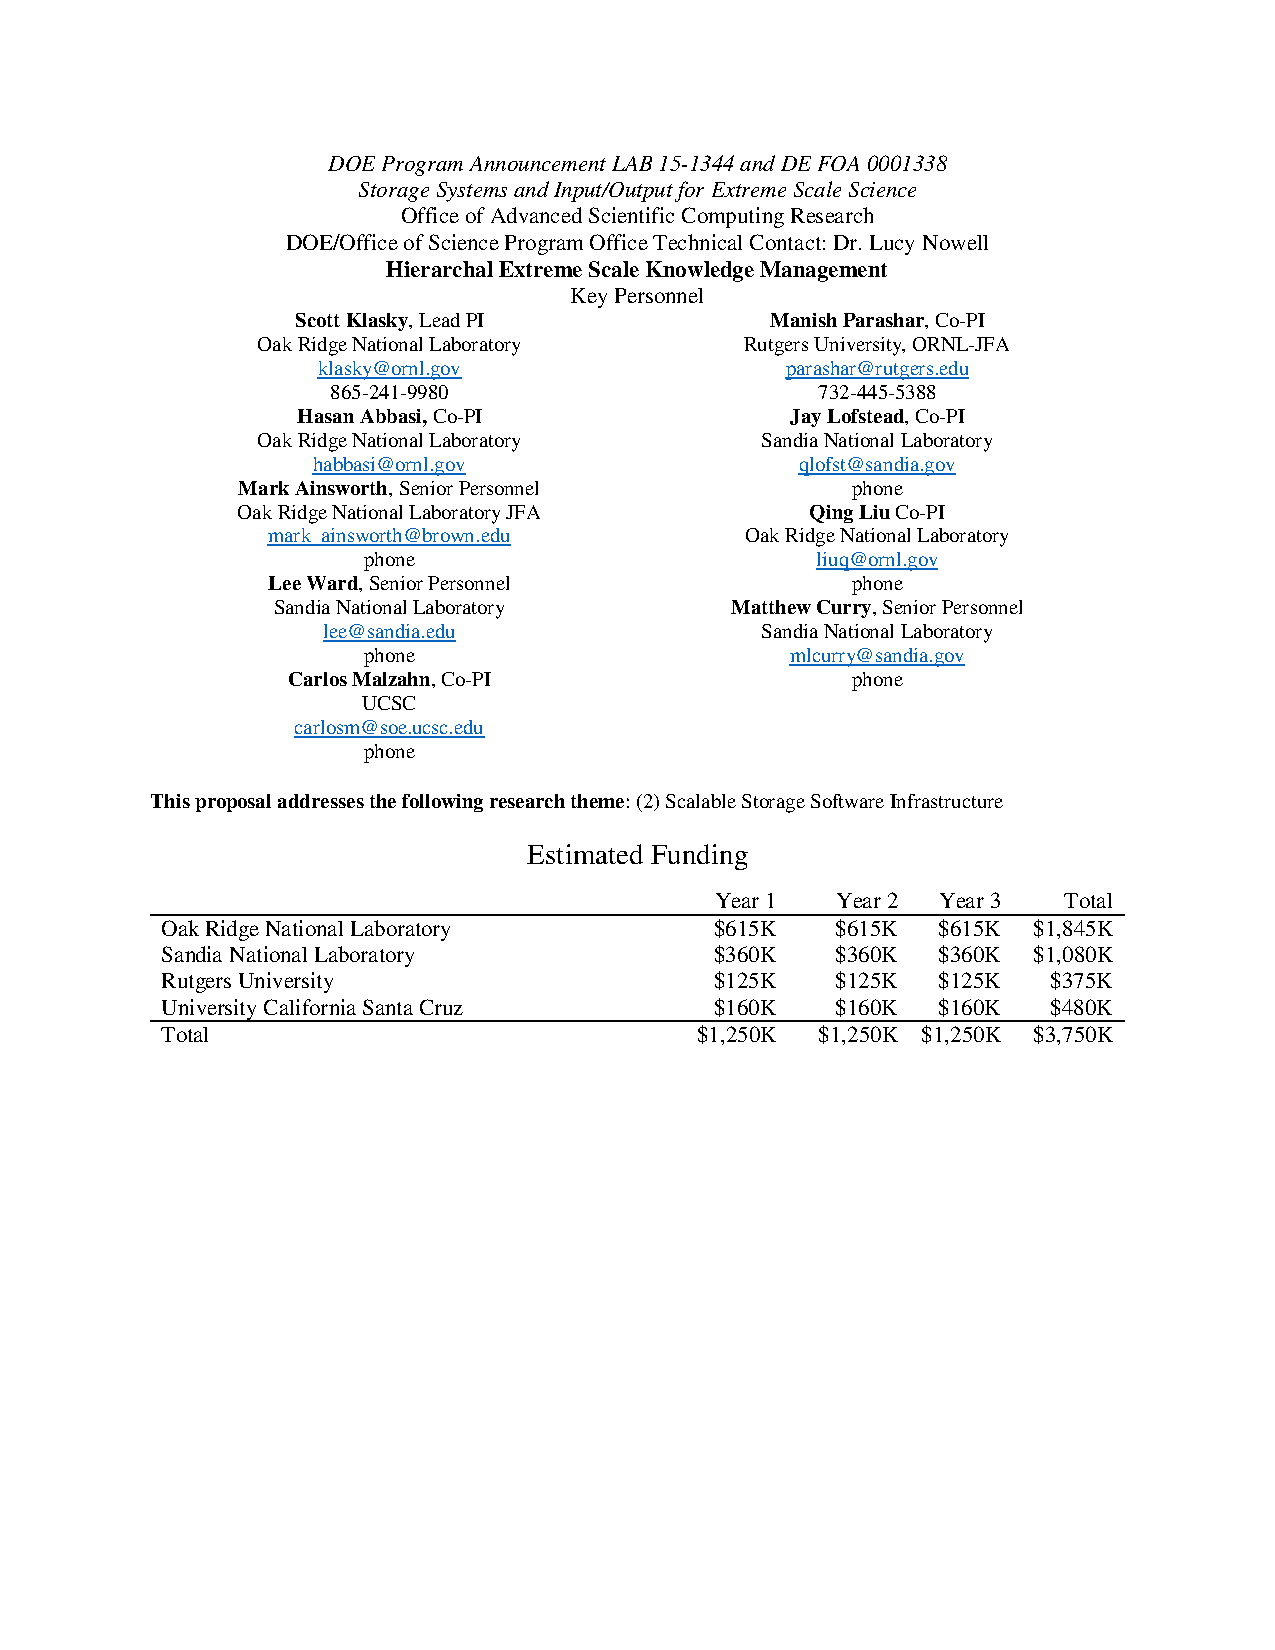
\includepdf[pages={1}]{ornl-cover.pdf}
%\pagebreak

\author{
  \IEEEauthorblockN {
    PI: Scott Klasky, % \IEEEauthorrefmark{1},
    Co-PI Manish Parashar % \IEEEauthorrefmark{1}
  }
  \IEEEauthorblockA {
    % \IEEEauthorrefmark{1}
    Mathematics and Computer Science Division,
    Argonne National Laboratory,
    Argonne, IL, USA}
}

%\maketitle

% Heilmeyer Points: from http://www.csee.umbc.edu/~finin/home/heilmeyerCatechism.html
% 
% \begin{enumerate}

% \item What is the problem, why is it hard? 

% \item How is it solved today?
%  Fig A: much 

% \item What is the new technical idea; why can we succeed now?
%  Integration of proven components into an architecure that solves
%  problems. New research will resolve remaining technical hurdles.

% \item What is the impact if successful?
%  Users and developers will be able to ...

% \item How will the program be organized?
%  Participants and focus areas

% \item How will intermediate results be generated?
%  Toolkit snapshots and application

% \item How will you measure progress?
%  Provide metrics

% \item What will it cost?
%  Cover sheet

% \end{enumerate}
%

{\bf Title of Pre-application:} Hierarchal Extreme Scale Knowledge Management \par
{\bf Principal Investigator:} Scott Klasky, Group Leader, ORNL, 854-241-9980, klasky@ornl.gov \par
{\bf Funding Opportunity Announcement Number: DE-FOA-0001338} \par
{\bf List of all co-PIs and Key/Senior Personnel} \par
Hasan Abbasi, Oak Ridge National Laboratory \par
Mark Ainsworth, Oak Ridge National Laboratory JFA, Brown University \par
Matthew Curry, Sandia National Laboratory\par
Qing Liu, Oak Ridge National Laboratory \par
Jay Lofstead, Sandia National Laboratory \par
Kimmy Mu, Oak Ridge National Laboratory \par
Carlos Malzahn, U. Cal. Santa Cruz \par
Manish Parashar, Rutgers University, Oak Ridge National Laboratory \par
 Sudharshan Vazhkudai, Oak Ridge National Laboratory \par
Lee Ward, Sandia National Laboratory \par
\vskip 0.2 in



\underline{\textbf{Objectives:}} Exascale scientific discovery will
introduce more complex hardware, and many simulations will be bottlenecked 
without sufficient new research into manging and storing the large data which will be
produced during the simulation, and analzyed for months after the simulations.
Our goal is to explore and address
the multi-tier challenges that are faced by scientists in creating and
managing and storing their data  to expedite insights into
mission critical scientific processes in exascale computing.
%
We propose a research program that aims to explore a hiearchical organization and storage infstraturure which will facilitiate 
how we data can be written and read efficiently. In order to help us explore our many research issues, we will build upon the
sucess of our middleware system, ADIOS, our multi-tier storage system, Sirocco, and our distributed storage system, Cepth.
We will also take advantage of our staging system, Data Spaces, and our Comon communication Interface (CCI) and build on all of
our sucessful software used in petascale simulations to understand the new directions which need to be understood to fully develop
the next generation I/O and Storage System for exascale and beyond systems.

%
We will apply a technique which will re-organize and possibly reduce the total amount of information based on user intentions along
with direct feedback from the storage and I/O system to allow data to be optimized not just for output, but also for many of the complex
reading patterns. Since data analysis and visualization will be performed in both an in situ and post processing environment, 
we will continue to use our I/O and storage abstractions to help enable applications to take full advantage of the hardware and softare 
environments. Because data volumes are strictly outstripping available bandwidths, compression will
be required. Rather than focusing solely on lossless compression, we will
incorporate lossy compression with the ability to annotate data allowing
optimized algorithm selection based on the numerical methods employed in the
source simulation. We plan to epxlore this tradeoff of storage capacity and
bandwidth for computation to determine how to offer the user options that can
meet their needs with desireable performance characteristics.
%
Our objective is to reduce the time to knowledge, which means that we will also support additional access modes, beyond the traditional 
Checkpoint/Restart methods, and understand that all data has errors associated with it and we will ensure that these become encoded to allow
for additional optimizations. For example, all scientific simulations contain approximations, and all measurements from obervations and experiments 
also contain errors. These errors can help guide how information can be presented to users, by allowing us to ask for information within a given 
accuracy bound, and also allow us to offer a mode for recomputation vs. data storage and reterival.  
%
{\bf: please list other things from UCSC, OLCF}.
%


\underline{\textbf{Key Technical Approach:}}
%We are fundamentally trying to address the fundmantal questions : 1)  How can we 
%place and mangage massive scienfici data across all of the tiers of the storage and memory
%hiearchy? 2) What are the proper semantics needed in order to help bring knowledge from the applications
%to the middleware layer. 3) What information from the storage layer can be exposed to the middleweare such
%that the placement of information can be agreed upon from what the application requires and what the
%system resources are available. 

Our approach will allow users to ``plug-in'' techniques to classify data, not as bytes but as motifs, where
we can understand relationships between objects (into data models) and relationships of data in variables.
This will allow us to adapt data from a variable into the various storage tiers. Rather than focus on simple data
compression, we will incoroarte a multitude of techniques to reduce data on the faster storage tiers, and keep the less
reduced information on the lower tiers.

We wish to support additional data access modes as well. First, within a given
accuracy bounds, offer a mode for recomputation from data stored in a ``fast''
tier to reduce data latencies. Second, exploratory analysis operations
frequently entail an overall data set view followed by targeted data
exploration based on identified features. We will offer support for a
configurable data access mode to support these sorts of analysis accesses. An
``overview'' access mode that gives a quick, approximate within error bounds,
data view that can guide feature selection offering rapid coarse-grained data
exploration without requiring loading the complete, detailed data set from
storage. Based on the granularity requested, the accuracy and size of the data
returned can be adjusted. At the most extreme setting, the original data can
be retrieved at the time cost of moving the potentially huge data quantity.
Third, to ensure available storage for subsequent operations, we will offer
automatic data migration based on user annotations for required data lifetimes
using monitoring and learning techniques. Unlike existing approaches, this will
be tempered both by the user annotations and through learned access patterns.
While past access patterns may not indicate future access because the
simulation run purpose may have changed, we are focused on scalability where
runs are subsequently larger as the simulation prepares for a capability run.
By learning from the output and access patterns during this run sequence, we
can accurate decide how to place and organize data for the critical capability
runs. Fourth, we anticipiate storing mutliple data copies, each compressed in
different ways according to the underlying media, some of these copies will
disappear based on storage pressures, but data persistence will be maintained
according to user specifications. Assuming a relatively low latency cache layer
before a tape system, we can offer exporatory data access reserving pulling
data from tape to just the data required. This will save scientists time and
make data stored on tape usable without long delays.

Our research efforts will be heavily focused on the need to, in a coordinated
manner, adapt data and metadata retention policies to the dynamic
resource balancing that will need to take place between the application,
OS/R, and hardware.

The success of this project will  provide insights into how to build middleware and storage layers which can interact
well with each other, and take user-provided hints. Today data is reduced by application scientist who have 
limited information on what the storage layer can provide. They often make comprimises based on this limited knowledge
and either tune their output for writing or reading performance. This data then gets moved to other locations, and much of
the tuning is lost when the data is read back during their post processing. Furthermore, there is a limited set of operations
which users will be able to stage to other staging nodes for real-tiime-reduction and visualization. 

We will identify,   through concrete application evaluation, the requirements for highly 
usable and scalable middleware and storage layers




%\includepdf[pages={1}]{COI.pdf}



\end{document}

%%% End: 
